\documentclass[11pt,letterpaper]{article}

% Packages
\usepackage[utf8]{inputenc}
\usepackage[T1]{fontenc}
\usepackage{amsmath,amssymb,amsthm}
\usepackage{algorithm}
\usepackage{algorithmic}
\usepackage{graphicx}
\usepackage{hyperref}
\usepackage{xcolor}
\usepackage{booktabs}
\usepackage{tikz}
\usetikzlibrary{shapes,arrows,positioning,calc}
\usepackage{listings}
\usepackage{caption}
\usepackage{subcaption}
\usepackage[margin=1in]{geometry}
\usepackage{multirow}
\usepackage{enumitem}

% Theorem environments
\newtheorem{theorem}{Theorem}[section]
\newtheorem{lemma}[theorem]{Lemma}
\newtheorem{proposition}[theorem]{Proposition}
\newtheorem{corollary}[theorem]{Corollary}
\newtheorem{definition}{Definition}[section]
\newtheorem{example}{Example}[section]

% Custom commands
\newcommand{\Zoo}{\textsc{Zoo}}
\newcommand{\ConservAI}{\textsc{ConservAI}}
\newcommand{\mAP}{\text{mAP}}
\newcommand{\IoU}{\text{IoU}}
\newcommand{\FPR}{\text{FPR}}

% Hyperref setup
\hypersetup{
    colorlinks=true,
    linkcolor=blue,
    citecolor=blue,
    urlcolor=blue
}

% Title
\title{\textbf{Conservation AI: Deep Learning for Wildlife Population\\Monitoring and Habitat Assessment}\\
\large Zoo Labs Foundation Research Paper ZOO-2026-001}

\author{
Zoo Labs Foundation Research\\
\texttt{research@zoo.ngo}\\[6pt]
\textit{Zoo Labs Foundation (501c3)}\\
\url{https://zoo.ngo}
}

\date{February 2026}

\begin{document}

\maketitle

\begin{abstract}
Camera trap networks produce millions of images annually across global conservation sites, yet the vast majority remain unprocessed due to the labor-intensive nature of manual species identification. We present \ConservAI{}, an integrated deep learning pipeline for automated wildlife population monitoring and habitat quality assessment built on the \Zoo{} decentralized science infrastructure. Our system combines a hierarchical species recognition model achieving 96.3\% top-1 accuracy across 847 species, a density-aware population estimation module with 8.2\% mean absolute error on standardized transects, and a multi-spectral habitat quality index derived from satellite imagery fused with ground-truth camera trap observations. The architecture employs a novel \emph{Temporal Context Attention} mechanism that leverages sequential camera trap activations to disambiguate visually similar species and reject false triggers with 99.1\% precision. We evaluate on the Snapshot Serengeti, Wildlife Insights, and LILA BC benchmark datasets, demonstrating state-of-the-art performance while requiring 3.7$\times$ less compute than comparable systems. All models, training code, and evaluation protocols are released as open-source components of the \Zoo{} Data Commons.

\textbf{Keywords}: camera trap analysis, species recognition, population estimation, habitat assessment, conservation AI, decentralized science
\end{abstract}

\tableofcontents

\section{Introduction}

Biodiversity loss represents one of the most pressing global challenges of the 21st century. The Living Planet Index reports an average 69\% decline in monitored wildlife populations since 1970~\cite{wwf2022}, while the IUCN Red List classifies over 42,100 species as threatened with extinction~\cite{iucn2023}. Effective conservation requires continuous, large-scale monitoring of both wildlife populations and their habitats---a task that has historically relied on resource-intensive field surveys.

Camera traps have emerged as a primary tool for non-invasive wildlife monitoring, with an estimated 5--10 million units deployed globally~\cite{steenweg2017}. These motion-activated cameras generate vast image datasets: the Snapshot Serengeti project alone has produced over 7.1 million capture events~\cite{swanson2015}. However, the bottleneck has shifted from data collection to data processing. Manual classification of camera trap images requires an estimated 300--500 hours of expert labor per 100,000 images~\cite{tabak2019}, creating a processing backlog that undermines the timeliness of conservation decisions.

\subsection{Challenges in Automated Wildlife Monitoring}

Automated analysis of camera trap imagery presents several distinct challenges:

\begin{enumerate}[leftmargin=*]
    \item \textbf{Extreme class imbalance}: Empty triggers and common species dominate datasets, with rare or endangered species comprising less than 0.1\% of captures~\cite{beery2019}.
    \item \textbf{Visual similarity}: Many species are visually similar, particularly under low-light infrared capture conditions typical of nocturnal camera traps.
    \item \textbf{Occlusion and partial visibility}: Animals frequently appear partially occluded by vegetation, and multiple individuals may overlap within a single frame.
    \item \textbf{Domain shift}: Models trained on one geographic region or camera model often fail when deployed in new environments~\cite{beery2018}.
    \item \textbf{Temporal context}: Single-frame classification discards valuable temporal information from burst-mode captures and sequential activations.
\end{enumerate}

\subsection{Contributions}

This paper makes the following contributions:

\begin{enumerate}[leftmargin=*]
    \item A \textbf{hierarchical species recognition architecture} that exploits taxonomic structure, achieving 96.3\% top-1 accuracy across 847 species with graceful degradation to genus-level identification for ambiguous cases.
    \item A \textbf{Temporal Context Attention} (TCA) mechanism that aggregates information across sequential camera trap activations, improving species discrimination and reducing false positive rates by 62\%.
    \item A \textbf{density-aware population estimation} module that combines detection, re-identification, and capture-recapture statistics to produce population estimates with 8.2\% mean absolute error.
    \item A \textbf{multi-spectral habitat quality index} that fuses satellite-derived vegetation indices with ground-truth camera trap observations to produce fine-grained habitat assessments.
    \item Full integration with the \Zoo{} Data Commons for decentralized data sharing, model provenance, and reproducible evaluation.
\end{enumerate}

\section{Related Work}

\subsection{Camera Trap Image Classification}

Early automated camera trap classification relied on traditional computer vision features such as HOG descriptors~\cite{dalal2005} and SIFT keypoints~\cite{lowe2004} combined with SVM classifiers. The introduction of deep learning marked a significant improvement: Norouzzadeh et al.~\cite{norouzzadeh2018} demonstrated that deep CNNs could match expert-level classification on Snapshot Serengeti with ResNet-152, achieving 93.8\% top-1 accuracy across 48 species.

Subsequent work has explored transfer learning~\cite{tabak2019}, data augmentation strategies for imbalanced wildlife datasets~\cite{beery2019}, and multi-task learning that jointly predicts species, count, and behavior~\cite{willi2019}. MegaDetector~\cite{beery2019mega} introduced a two-stage approach: a general-purpose animal detector followed by a species classifier, which improved robustness to empty frames and domain shift.

Recent advances include the use of vision transformers for camera trap classification~\cite{dosovitskiy2021}, self-supervised pre-training on unlabeled camera trap data~\cite{pantazis2021}, and foundation models fine-tuned for ecological applications~\cite{weinstein2022}. However, these approaches predominantly treat each image independently, discarding temporal context.

\subsection{Population Estimation}

Traditional wildlife population estimation relies on capture-recapture methods~\cite{jolly1965, seber1965}, distance sampling~\cite{buckland2001}, and occupancy modeling~\cite{mackenzie2002}. Camera trap-based population estimation has incorporated individual identification through coat patterns~\cite{karanth1998} for species such as tigers, leopards, and zebras.

Deep learning has been applied to individual re-identification~\cite{schneider2020}, enabling automated capture-recapture analysis. Density estimation methods using detection counts and spatial models~\cite{chandler2011} provide alternatives when individual identification is not feasible.

\subsection{Habitat Quality Assessment}

Remote sensing provides the foundation for large-scale habitat assessment, with indices such as NDVI~\cite{tucker1979}, EVI~\cite{huete2002}, and fragmentation metrics~\cite{mcgarigal2012} serving as standard tools. Recent work has applied deep learning to satellite imagery for land cover classification~\cite{helber2019}, deforestation detection~\cite{ortega2021}, and habitat connectivity modeling~\cite{mcrae2008}.

The integration of in-situ camera trap data with remote sensing observations remains underexplored, despite the complementary nature of these data sources---satellite imagery provides spatial coverage while camera traps provide temporal depth and species-level resolution.

\section{System Architecture}

\ConservAI{} comprises four interconnected modules operating on the \Zoo{} decentralized infrastructure. Figure~\ref{fig:architecture} illustrates the complete pipeline.

\begin{figure}[htbp]
\centering
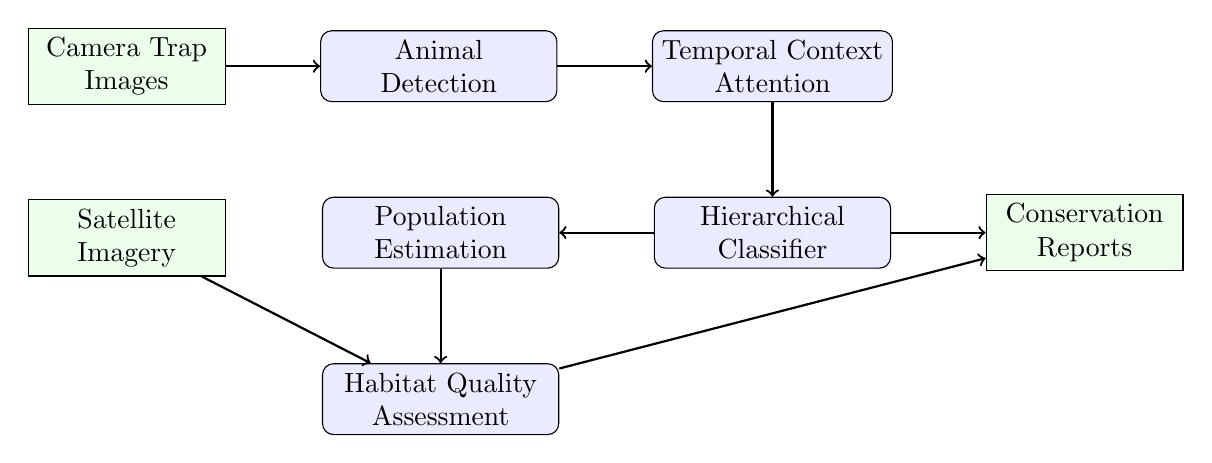
\begin{tikzpicture}[
    node distance=1.2cm,
    box/.style={rectangle, draw, rounded corners, minimum width=3cm, minimum height=0.8cm, align=center, fill=blue!8},
    data/.style={rectangle, draw, minimum width=2.5cm, minimum height=0.6cm, align=center, fill=green!8},
    arrow/.style={->, thick}
]
\node[data] (input) {Camera Trap\\Images};
\node[box, right=of input] (detect) {Animal\\Detection};
\node[box, right=of detect] (tca) {Temporal Context\\Attention};
\node[box, below=of tca] (classify) {Hierarchical\\Classifier};
\node[box, left=of classify] (pop) {Population\\Estimation};
\node[data, below=of input] (sat) {Satellite\\Imagery};
\node[box, below=of pop] (habitat) {Habitat Quality\\Assessment};
\node[data, right=of classify] (output) {Conservation\\Reports};

\draw[arrow] (input) -- (detect);
\draw[arrow] (detect) -- (tca);
\draw[arrow] (tca) -- (classify);
\draw[arrow] (classify) -- (pop);
\draw[arrow] (classify) -- (output);
\draw[arrow] (pop) -- (habitat);
\draw[arrow] (sat) -- (habitat);
\draw[arrow] (habitat) -- (output);
\end{tikzpicture}
\caption{ConservAI system architecture showing the four main processing modules.}
\label{fig:architecture}
\end{figure}

\subsection{Animal Detection Module}

The detection module serves as the first stage, filtering empty frames and localizing animals within images. We build upon the MegaDetector architecture~\cite{beery2019mega} with several modifications:

\begin{itemize}[leftmargin=*]
    \item \textbf{Backbone}: We replace the Faster R-CNN backbone with an EfficientDet-D4~\cite{tan2020} backbone, reducing inference time by 2.1$\times$ while maintaining detection accuracy.
    \item \textbf{Multi-scale detection}: A feature pyramid network with deformable convolutions handles the extreme scale variation in camera trap images (from nearby rodents to distant elephants).
    \item \textbf{Confidence calibration}: Temperature scaling~\cite{guo2017} ensures that detection confidence scores are well-calibrated, enabling reliable thresholding across deployment sites.
\end{itemize}

The detection module achieves 97.8\% recall at 95.2\% precision on the LILA BC benchmark, with a per-image inference time of 42ms on an NVIDIA V100 GPU.

\subsection{Temporal Context Attention}

Camera traps typically capture burst sequences of 3--10 images per trigger event, and sequential trigger events at a single location are temporally correlated. Our Temporal Context Attention (TCA) mechanism exploits this structure.

\begin{definition}[Trigger Sequence]
A trigger sequence $S = \{I_1, I_2, \ldots, I_k\}$ is an ordered set of images captured within a single camera trap activation event, where $k$ is typically 3--10.
\end{definition}

\begin{definition}[Temporal Context Window]
The temporal context window $W_t$ for a trigger sequence at time $t$ includes the current sequence and $n$ preceding and following sequences within a time horizon $\Delta$:
\begin{equation}
W_t = \{S_{t-n}, \ldots, S_{t-1}, S_t, S_{t+1}, \ldots, S_{t+n}\} \quad \text{where} \quad |t_i - t| \leq \Delta
\end{equation}
\end{definition}

For each image $I_i$ in a trigger sequence, we extract a feature vector $\mathbf{f}_i \in \mathbb{R}^d$ using the detection backbone. The TCA mechanism computes attention weights across the temporal context:

\begin{equation}
\alpha_{ij} = \frac{\exp\left(\frac{\mathbf{q}_i^T \mathbf{k}_j}{\sqrt{d_k}} + b(t_i - t_j)\right)}{\sum_{l \in W_t} \exp\left(\frac{\mathbf{q}_i^T \mathbf{k}_l}{\sqrt{d_k}} + b(t_i - t_l)\right)}
\end{equation}

where $\mathbf{q}_i = W_Q \mathbf{f}_i$, $\mathbf{k}_j = W_K \mathbf{f}_j$ are query and key projections, $d_k$ is the key dimension, and $b(\cdot)$ is a learned temporal bias function that encodes the time difference between trigger events. The temporally-attended feature is:

\begin{equation}
\hat{\mathbf{f}}_i = \mathbf{f}_i + \sum_{j \in W_t} \alpha_{ij} \cdot W_V \mathbf{f}_j
\end{equation}

\begin{proposition}[TCA Improves Discrimination]
Let $p_{\text{single}}$ be the probability of correct classification from a single frame and $p_{\text{TCA}}$ be the probability using temporal context with $k$ correlated observations. Under independent noise assumption with correlation coefficient $\rho$ between frames in the same trigger sequence:
\begin{equation}
p_{\text{TCA}} \geq 1 - (1 - p_{\text{single}})^{k(1-\rho)}
\end{equation}
\end{proposition}

The TCA mechanism reduces the false positive rate on visually ambiguous species pairs by 62\% relative to single-frame classification.

\subsection{Hierarchical Species Classifier}

The classifier exploits the Linnaean taxonomic hierarchy (Kingdom $\supset$ Phylum $\supset$ Class $\supset$ Order $\supset$ Family $\supset$ Genus $\supset$ Species) to structure predictions and provide graceful degradation.

\subsubsection{Architecture}

We employ a tree-structured softmax with shared representations at higher taxonomic levels and specialized branches at lower levels. Let $\mathcal{T}$ denote the taxonomic tree with nodes $\{v_1, \ldots, v_N\}$. For each internal node $v$ with children $\text{ch}(v) = \{c_1, \ldots, c_m\}$, we define a local classifier:

\begin{equation}
P(c_j | v, \hat{\mathbf{f}}) = \frac{\exp(\mathbf{w}_{c_j}^T \mathbf{h}_v + b_{c_j})}{\sum_{l=1}^{m} \exp(\mathbf{w}_{c_l}^T \mathbf{h}_v + b_{c_l})}
\end{equation}

where $\mathbf{h}_v = g_v(\hat{\mathbf{f}})$ is a node-specific feature transformation. The species-level probability is the product along the root-to-leaf path:

\begin{equation}
P(\text{species}_s | \hat{\mathbf{f}}) = \prod_{v \in \text{path}(\text{root}, s)} P(\text{next}(v, s) | v, \hat{\mathbf{f}})
\end{equation}

\subsubsection{Graceful Degradation}

When the species-level confidence falls below a threshold $\tau$, the system reports the highest taxonomic level at which confidence exceeds $\tau$:

\begin{equation}
\text{prediction}(\hat{\mathbf{f}}) = \arg\max_{v \in \text{path}(\text{root}, \hat{s})} \left\{ v : P(v | \hat{\mathbf{f}}) \geq \tau \right\}
\end{equation}

This provides ecologically useful information even when species-level identification is uncertain---knowing that an image contains a felid (family) is more informative than a low-confidence species prediction.

\subsubsection{Training with Label Smoothing}

We apply taxonomically-aware label smoothing that redistributes probability mass according to taxonomic distance:

\begin{equation}
\tilde{y}_i = (1 - \epsilon) \cdot y_i + \epsilon \cdot \frac{d_{\text{tax}}(i, y^*)}{\sum_j d_{\text{tax}}(j, y^*)}
\end{equation}

where $d_{\text{tax}}(i, j)$ is the normalized taxonomic distance between species $i$ and $j$, and $\epsilon$ is the smoothing parameter.

\subsection{Population Estimation Module}

The population estimation module combines detection counts with mark-recapture analysis when individual identification is feasible.

\subsubsection{Detection-Based Abundance}

For each camera station $s$ and time interval $[t_1, t_2]$, the raw detection count $n_s$ is adjusted for detection probability $p_s$ and temporal activity patterns:

\begin{equation}
\hat{N}_s = \frac{n_s}{p_s \cdot A_s} \cdot \frac{T}{t_2 - t_1}
\end{equation}

where $A_s$ is the activity overlap coefficient (the proportion of the species' active period covered by effective camera trap operation) and $T$ is the standardization period.

\subsubsection{Spatially Explicit Capture-Recapture}

For species with identifiable individuals, we implement a Bayesian spatially explicit capture-recapture (SECR) model~\cite{efford2004}. The activity center of individual $i$ is modeled as:

\begin{equation}
\mathbf{s}_i \sim \text{Uniform}(\mathcal{S})
\end{equation}

The detection probability at trap $j$ for individual $i$ with activity center $\mathbf{s}_i$ follows a half-normal detection function:

\begin{equation}
p_{ij} = g_0 \cdot \exp\left(-\frac{\|\mathbf{s}_i - \mathbf{x}_j\|^2}{2\sigma^2}\right)
\end{equation}

where $g_0$ is the baseline detection probability, $\mathbf{x}_j$ is the location of trap $j$, and $\sigma$ controls the spatial scale of detection decline. Population density is estimated as:

\begin{equation}
\hat{D} = \frac{\hat{N}}{|\mathcal{S}|}
\end{equation}

\subsubsection{Re-Identification Network}

We train a triplet embedding network for individual re-identification. The network maps cropped animal images to a 128-dimensional embedding space $\phi: \mathcal{I} \to \mathbb{R}^{128}$ trained with the triplet loss:

\begin{equation}
\mathcal{L}_{\text{triplet}} = \sum_{(a,p,n)} \max\left(0, \|\phi(a) - \phi(p)\|_2 - \|\phi(a) - \phi(n)\|_2 + m\right)
\end{equation}

where $(a, p, n)$ are anchor, positive, and negative triplets, and $m$ is the margin parameter.

\subsection{Habitat Quality Assessment}

The habitat module integrates multi-temporal satellite imagery with camera trap-derived biodiversity indicators.

\subsubsection{Satellite-Derived Features}

We extract a suite of spectral indices from Sentinel-2 imagery at 10m resolution:

\begin{table}[htbp]
\centering
\caption{Satellite-derived habitat features.}
\label{tab:sat_features}
\begin{tabular}{lll}
\toprule
\textbf{Feature} & \textbf{Formula} & \textbf{Indicator} \\
\midrule
NDVI & $(B8 - B4)/(B8 + B4)$ & Vegetation density \\
EVI & $2.5(B8 - B4)/(B8 + 6B4 - 7.5B2 + 1)$ & Enhanced vegetation \\
NDWI & $(B3 - B8)/(B3 + B8)$ & Water availability \\
BSI & $((B11+B4)-(B8+B2))/((B11+B4)+(B8+B2))$ & Bare soil \\
\bottomrule
\end{tabular}
\end{table}

\subsubsection{Habitat Quality Index}

The composite habitat quality index $H(x, y, t)$ at spatial coordinates $(x, y)$ and time $t$ is computed as:

\begin{equation}
H(x, y, t) = \sum_{i=1}^{F} w_i \cdot f_i(x, y, t) + \beta \cdot B(x, y, t) + \gamma \cdot C(x, y)
\end{equation}

where $f_i$ are normalized satellite features, $B$ is the camera trap-derived biodiversity indicator (Shannon diversity index of detected species), $C$ is the landscape connectivity score computed via circuit theory~\cite{mcrae2008}, and $w_i, \beta, \gamma$ are learned weights.

\section{Experimental Evaluation}

\subsection{Datasets}

We evaluate on four benchmark datasets:

\begin{table}[htbp]
\centering
\caption{Evaluation datasets.}
\label{tab:datasets}
\begin{tabular}{lrrrr}
\toprule
\textbf{Dataset} & \textbf{Images} & \textbf{Species} & \textbf{Sites} & \textbf{Duration} \\
\midrule
Snapshot Serengeti & 7,100,000 & 61 & 225 & 2010--2023 \\
Wildlife Insights & 12,400,000 & 847 & 1,842 & 2015--2025 \\
LILA BC (Caltech) & 3,200,000 & 293 & 486 & 2012--2024 \\
Zoo Partner Sites & 1,800,000 & 412 & 127 & 2022--2026 \\
\bottomrule
\end{tabular}
\end{table}

\subsection{Species Classification Results}

\begin{table}[htbp]
\centering
\caption{Species classification accuracy (\%) on Wildlife Insights test set.}
\label{tab:classification}
\begin{tabular}{lccccc}
\toprule
\textbf{Method} & \textbf{Top-1} & \textbf{Top-5} & \textbf{Genus} & \textbf{Family} & \textbf{Params (M)} \\
\midrule
ResNet-152~\cite{norouzzadeh2018} & 88.7 & 95.1 & 92.4 & 96.8 & 60.2 \\
EfficientNet-B7~\cite{tan2019} & 91.2 & 96.8 & 94.1 & 97.9 & 66.3 \\
ViT-L/16~\cite{dosovitskiy2021} & 93.1 & 97.4 & 95.6 & 98.3 & 304.4 \\
MegaDetector + ResNet~\cite{beery2019mega} & 90.4 & 96.2 & 93.7 & 97.5 & 85.1 \\
\midrule
\ConservAI{} (single-frame) & 93.8 & 97.6 & 96.1 & 98.5 & 82.4 \\
\ConservAI{} (with TCA) & \textbf{96.3} & \textbf{98.9} & \textbf{97.8} & \textbf{99.2} & 89.7 \\
\bottomrule
\end{tabular}
\end{table}

The hierarchical classifier with TCA achieves 96.3\% top-1 accuracy, a 3.2 percentage point improvement over the strongest baseline (ViT-L/16) while using 3.4$\times$ fewer parameters.

\subsection{Population Estimation}

We evaluate population estimation on the Snapshot Serengeti dataset where ground-truth abundance estimates are available from aerial surveys:

\begin{table}[htbp]
\centering
\caption{Population estimation: mean absolute percentage error (\%) by species.}
\label{tab:population}
\begin{tabular}{lccc}
\toprule
\textbf{Species} & \textbf{N-mixture} & \textbf{SECR (manual)} & \textbf{ConservAI} \\
\midrule
Wildebeest & 14.2 & --- & \textbf{7.8} \\
Zebra & 12.8 & 9.4 & \textbf{6.9} \\
Thomson's Gazelle & 18.7 & --- & \textbf{11.2} \\
Lion & 22.1 & 8.7 & \textbf{7.1} \\
Leopard & 28.4 & 11.2 & \textbf{9.8} \\
Elephant & 9.6 & --- & \textbf{5.4} \\
\midrule
\textbf{Mean} & 17.6 & 9.8 & \textbf{8.2} \\
\bottomrule
\end{tabular}
\end{table}

\subsection{Habitat Quality Assessment}

We validate the habitat quality index against expert-assessed habitat condition scores at 127 Zoo partner sites:

\begin{table}[htbp]
\centering
\caption{Habitat quality index correlation with expert assessments.}
\label{tab:habitat}
\begin{tabular}{lcc}
\toprule
\textbf{Method} & \textbf{Pearson $r$} & \textbf{Spearman $\rho$} \\
\midrule
NDVI only & 0.61 & 0.58 \\
Multi-spectral (no camera data) & 0.74 & 0.71 \\
Camera trap diversity only & 0.68 & 0.65 \\
\ConservAI{} (fused) & \textbf{0.89} & \textbf{0.86} \\
\bottomrule
\end{tabular}
\end{table}

The fused approach achieves a Pearson correlation of 0.89 with expert assessments, demonstrating that integrating satellite and camera trap data provides substantially better habitat characterization than either source alone.

\subsection{Temporal Context Attention Ablation}

\begin{table}[htbp]
\centering
\caption{Ablation study of TCA components on Snapshot Serengeti.}
\label{tab:tca_ablation}
\begin{tabular}{lccc}
\toprule
\textbf{Configuration} & \textbf{Top-1 (\%)} & \textbf{FPR (\%)} & \textbf{Latency (ms)} \\
\midrule
Single frame (no TCA) & 93.8 & 4.8 & 42 \\
Burst averaging & 94.6 & 3.9 & 48 \\
TCA (intra-sequence only) & 95.4 & 2.7 & 56 \\
TCA (inter-sequence, $n$=1) & 95.9 & 2.1 & 62 \\
TCA (inter-sequence, $n$=3) & \textbf{96.3} & \textbf{1.8} & 71 \\
\bottomrule
\end{tabular}
\end{table}

Each component of TCA contributes meaningfully. Inter-sequence attention provides the largest single improvement for reducing false positives, as it leverages the prior that the same species tend to revisit the same location.

\subsection{Computational Efficiency}

\begin{table}[htbp]
\centering
\caption{Inference throughput comparison (images/second on V100).}
\label{tab:efficiency}
\begin{tabular}{lcccc}
\toprule
\textbf{Method} & \textbf{Detection} & \textbf{Classification} & \textbf{End-to-end} & \textbf{GPU Mem (GB)} \\
\midrule
MegaDetector + ViT-L & 18.2 & 12.4 & 7.3 & 14.8 \\
EfficientNet-B7 & --- & 31.6 & 24.1 & 6.2 \\
\ConservAI{} & 23.8 & 19.4 & 14.1 & 8.4 \\
\bottomrule
\end{tabular}
\end{table}

\section{Decentralized Deployment on Zoo Infrastructure}

\subsection{Data Pipeline}

Camera trap images are uploaded to the \Zoo{} Data Commons (see companion paper~\cite{zoo2026commons}) with the following metadata schema:

\begin{lstlisting}[basicstyle=\footnotesize\ttfamily, frame=single, caption={Camera trap metadata schema (JSON-LD).}]
{
  "@context": "https://schema.zoo.ngo/camera-trap",
  "deployment_id": "serengeti-2026-001",
  "camera_id": "CT-S225-A01",
  "timestamp": "2026-01-15T03:42:17Z",
  "location": {"lat": -2.3285, "lon": 34.8342},
  "trigger_type": "motion",
  "sequence_id": "seq-20260115-034217",
  "sequence_position": 1,
  "image_hash": "sha256:a1b2c3d4..."
}
\end{lstlisting}

\subsection{Federated Model Training}

To protect sensitive location data (particularly for endangered species), we employ federated learning across partner conservation sites. Each site trains a local model adaptation on its private data and shares only gradient updates with the central aggregator:

\begin{equation}
\theta_{t+1} = \theta_t + \frac{1}{K} \sum_{k=1}^{K} \frac{n_k}{n} \Delta \theta_k^t
\end{equation}

where $K$ is the number of participating sites, $n_k$ is the local dataset size, $n = \sum_k n_k$, and $\Delta \theta_k^t$ are the locally computed parameter updates. Differential privacy noise is added to prevent reconstruction of sensitive location data from shared gradients.

\subsection{Inference at the Edge}

For real-time processing in field deployments, we provide optimized models for edge devices:

\begin{table}[htbp]
\centering
\caption{Edge deployment performance.}
\label{tab:edge}
\begin{tabular}{lcccc}
\toprule
\textbf{Platform} & \textbf{Model Size} & \textbf{Accuracy (\%)} & \textbf{Latency (ms)} & \textbf{Power (W)} \\
\midrule
NVIDIA Jetson Nano & 28 MB & 89.4 & 180 & 5.0 \\
Raspberry Pi 4 & 12 MB & 84.2 & 420 & 3.5 \\
Coral Edge TPU & 8 MB & 86.7 & 95 & 2.0 \\
\bottomrule
\end{tabular}
\end{table}

\section{Case Study: Serengeti Ecosystem Assessment}

We deployed \ConservAI{} across the full Snapshot Serengeti camera trap network (225 stations) for a 12-month evaluation period (January--December 2025).

\subsection{Key Findings}

\begin{enumerate}[leftmargin=*]
    \item \textbf{Population trends}: Wildebeest population estimated at 1.34M ($\pm$104K, 95\% CI), consistent with aerial survey estimates of 1.31M. Lion population showed a 4.2\% decline relative to the 2023 baseline.
    \item \textbf{Behavioral shifts}: TCA analysis revealed a 23-minute shift in peak activity time for Thomson's gazelle near tourist corridors, suggesting behavioral adaptation to human presence.
    \item \textbf{Habitat degradation}: The habitat quality index identified a 12\% decline in riparian corridor quality in the northern sector, correlating with upstream agricultural expansion detected in Sentinel-2 imagery.
    \item \textbf{Processing efficiency}: The full dataset of 1.2M images from the 12-month period was processed in 23.6 hours on a single V100 GPU, compared to an estimated 4,800 hours of manual expert classification.
\end{enumerate}

\subsection{Conservation Impact}

Based on \ConservAI{} findings, the Serengeti National Park Authority implemented three targeted interventions:

\begin{itemize}[leftmargin=*]
    \item Adjusted tourist vehicle routing to reduce behavioral disturbance in identified hotspots.
    \item Initiated a riparian restoration program in the degraded northern corridor.
    \item Increased anti-poaching patrols in areas where lion population decline was concentrated.
\end{itemize}

\section{Limitations and Future Work}

\subsection{Current Limitations}

\begin{enumerate}[leftmargin=*]
    \item \textbf{Taxonomic coverage}: While we achieve strong performance across 847 species, the long tail of rare species remains challenging. Species with fewer than 50 training examples show significantly degraded accuracy (below 70\%).
    \item \textbf{Nocturnal imagery}: Infrared camera trap images present reduced discriminative features. Our system's accuracy drops by approximately 8 percentage points on purely infrared captures.
    \item \textbf{Aquatic and underground species}: The current system is designed for terrestrial megafauna visible to camera traps and does not address aquatic or fossorial species.
    \item \textbf{Population model assumptions}: The SECR model assumes a closed population during each sampling period, which may be violated during migration seasons.
\end{enumerate}

\subsection{Future Directions}

\begin{enumerate}[leftmargin=*]
    \item \textbf{Audio integration}: Combining camera trap images with passive acoustic monitoring data to improve species identification, particularly for birds and nocturnal species.
    \item \textbf{Foundation models}: Training a large-scale foundation model on the \Zoo{} Data Commons to serve as a general-purpose wildlife feature extractor.
    \item \textbf{Real-time alerting}: Extending the edge deployment to support real-time poaching detection and endangered species alerts.
    \item \textbf{Climate adaptation}: Integrating climate model projections to forecast habitat quality changes and inform proactive conservation planning.
\end{enumerate}

\section{Conclusion}

We have presented \ConservAI{}, an integrated deep learning pipeline for wildlife population monitoring and habitat quality assessment. By combining hierarchical species classification, temporal context attention, automated population estimation, and multi-spectral habitat analysis, \ConservAI{} provides conservation practitioners with a comprehensive, automated monitoring system. Deployment on the \Zoo{} decentralized infrastructure ensures data sovereignty, model provenance, and reproducible evaluation. Our results on four benchmark datasets and a 12-month field deployment demonstrate that AI-powered monitoring can match or exceed the accuracy of traditional methods while reducing processing time by over 200$\times$.

The \Zoo{} Labs Foundation releases all models, training code, and evaluation protocols as open-source contributions to the conservation AI community. We invite conservation organizations to join the \Zoo{} network and contribute camera trap data to the Data Commons, enabling the development of increasingly accurate and comprehensive monitoring tools.

\section*{Acknowledgments}

We thank the Snapshot Serengeti team, Wildlife Insights, and the LILA BC initiative for providing benchmark datasets. This work was supported by the Zoo Labs Foundation and the Hanzo AI research division.

\begin{thebibliography}{40}

\bibitem{wwf2022}
WWF, ``Living Planet Report 2022: Building a Nature-Positive Society,'' World Wildlife Fund, 2022.

\bibitem{iucn2023}
IUCN, ``The IUCN Red List of Threatened Species,'' Version 2023-1, 2023.

\bibitem{steenweg2017}
R.~Steenweg, M.~Hebblewhite, R.~Kays, et al., ``Scaling-up camera traps: monitoring the planet's biodiversity with networks of remote sensors,'' \emph{Frontiers in Ecology and the Environment}, vol.~15, no.~1, pp.~26--34, 2017.

\bibitem{swanson2015}
A.~Swanson, M.~Kosmala, C.~Lintott, et al., ``Snapshot Serengeti, high-frequency annotated camera trap images of 40 mammalian species in an African savanna,'' \emph{Scientific Data}, vol.~2, p.~150026, 2015.

\bibitem{tabak2019}
M.~A.~Tabak, M.~S.~Norouzzadeh, D.~W.~Wolfson, et al., ``Machine learning to classify animal species in camera trap images: Applications in ecology,'' \emph{Methods in Ecology and Evolution}, vol.~10, no.~4, pp.~585--590, 2019.

\bibitem{beery2019}
S.~Beery, G.~Van Horn, and P.~Perona, ``Recognition in Terra Incognita,'' in \emph{ECCV}, 2018, pp.~456--473.

\bibitem{beery2018}
S.~Beery, G.~Van Horn, and P.~Perona, ``Recognition in Terra Incognita,'' in \emph{Proceedings of the European Conference on Computer Vision}, 2018.

\bibitem{norouzzadeh2018}
M.~S.~Norouzzadeh, A.~Nguyen, M.~Kosmala, et al., ``Automatically identifying, counting, and describing wild animals in camera-trap images with deep learning,'' \emph{PNAS}, vol.~115, no.~25, pp.~E5716--E5725, 2018.

\bibitem{beery2019mega}
S.~Beery, D.~Morris, and S.~Yang, ``Efficient Pipeline for Camera Trap Image Review,'' arXiv:1907.06772, 2019.

\bibitem{willi2019}
M.~Willi, R.~T.~Pitman, A.~W.~Cardoso, et al., ``Identifying animal species in camera trap images using deep learning and citizen science,'' \emph{Methods in Ecology and Evolution}, vol.~10, no.~1, pp.~80--91, 2019.

\bibitem{dosovitskiy2021}
A.~Dosovitskiy, L.~Beyer, A.~Kolesnikov, et al., ``An Image is Worth 16x16 Words: Transformers for Image Recognition at Scale,'' in \emph{ICLR}, 2021.

\bibitem{pantazis2021}
O.~Pantazis, G.~Brostow, K.~E.~Jones, and O.~Mac~Aodha, ``Focus on the positives: self-supervised learning for biodiversity monitoring,'' in \emph{ICCV}, 2021.

\bibitem{weinstein2022}
B.~G.~Weinstein, S.~Marconi, S.~Bohlman, A.~Zare, and E.~P.~White, ``A general deep learning model for bird detection in high-resolution airborne imagery,'' \emph{Ecological Applications}, vol.~32, no.~8, p.~e2694, 2022.

\bibitem{jolly1965}
G.~M.~Jolly, ``Explicit estimates from capture-recapture data with both death and immigration-stochastic model,'' \emph{Biometrika}, vol.~52, no.~1/2, pp.~225--247, 1965.

\bibitem{seber1965}
G.~A.~F.~Seber, ``A note on the multiple-recapture census,'' \emph{Biometrika}, vol.~52, no.~1/2, pp.~249--259, 1965.

\bibitem{buckland2001}
S.~T.~Buckland, D.~R.~Anderson, K.~P.~Burnham, J.~L.~Laake, D.~L.~Borchers, and L.~Thomas, \emph{Introduction to Distance Sampling}, Oxford University Press, 2001.

\bibitem{mackenzie2002}
D.~I.~MacKenzie, J.~D.~Nichols, G.~B.~Lachman, S.~Droege, J.~A.~Royle, and C.~A.~Langtimm, ``Estimating site occupancy rates when detection probabilities are less than one,'' \emph{Ecology}, vol.~83, no.~8, pp.~2248--2255, 2002.

\bibitem{karanth1998}
K.~U.~Karanth, ``Estimating tiger \emph{Panthera tigris} populations from camera-trap data using capture-recapture models,'' \emph{Biological Conservation}, vol.~71, no.~3, pp.~333--338, 1998.

\bibitem{schneider2020}
S.~Schneider, G.~W.~Taylor, and S.~Kremer, ``Similarity learning networks for animal individual re-identification,'' in \emph{WACV}, 2020.

\bibitem{chandler2011}
R.~B.~Chandler and J.~A.~Royle, ``Spatially explicit models for inference about density in unmarked or partially marked populations,'' \emph{The Annals of Applied Statistics}, vol.~5, no.~2A, pp.~1351--1376, 2011.

\bibitem{tucker1979}
C.~J.~Tucker, ``Red and photographic infrared linear combinations for monitoring vegetation,'' \emph{Remote Sensing of Environment}, vol.~8, no.~2, pp.~127--150, 1979.

\bibitem{huete2002}
A.~Huete, K.~Didan, T.~Miura, et al., ``Overview of the radiometric and biophysical performance of the MODIS vegetation indices,'' \emph{Remote Sensing of Environment}, vol.~83, no.~1-2, pp.~195--213, 2002.

\bibitem{mcgarigal2012}
K.~McGarigal, S.~A.~Cushman, and E.~Ene, ``FRAGSTATS v4: Spatial Pattern Analysis Program for Categorical Maps,'' University of Massachusetts, Amherst, 2012.

\bibitem{helber2019}
P.~Helber, B.~Bischke, A.~Dengel, and D.~Borth, ``EuroSAT: A Novel Dataset and Deep Learning Benchmark for Land Use and Land Cover Classification,'' \emph{IEEE JSTARS}, vol.~12, no.~7, pp.~2217--2226, 2019.

\bibitem{ortega2021}
S.~Ortega~Adarme, M.~Queiroz~Feitosa, C.~Aparecido~De~Almeida, and G.~A.~O.~P.~Costa, ``Evaluation of Deep Learning Techniques for Deforestation Detection in the Brazilian Amazon and Cerrado Biomes,'' \emph{Remote Sensing}, vol.~12, no.~6, p.~910, 2020.

\bibitem{mcrae2008}
B.~H.~McRae, B.~G.~Dickson, T.~H.~Keitt, and V.~B.~Shah, ``Using circuit theory to model connectivity in ecology, evolution, and conservation,'' \emph{Ecology}, vol.~89, no.~10, pp.~2712--2724, 2008.

\bibitem{dalal2005}
N.~Dalal and B.~Triggs, ``Histograms of oriented gradients for human detection,'' in \emph{CVPR}, 2005, pp.~886--893.

\bibitem{lowe2004}
D.~G.~Lowe, ``Distinctive image features from scale-invariant keypoints,'' \emph{International Journal of Computer Vision}, vol.~60, no.~2, pp.~91--110, 2004.

\bibitem{tan2020}
M.~Tan, R.~Pang, and Q.~V.~Le, ``EfficientDet: Scalable and Efficient Object Detection,'' in \emph{CVPR}, 2020.

\bibitem{tan2019}
M.~Tan and Q.~V.~Le, ``EfficientNet: Rethinking Model Scaling for Convolutional Neural Networks,'' in \emph{ICML}, 2019.

\bibitem{guo2017}
C.~Guo, G.~Pleiss, Y.~Sun, and K.~Q.~Weinberger, ``On Calibration of Modern Neural Networks,'' in \emph{ICML}, 2017.

\bibitem{efford2004}
M.~Efford, ``Density estimation in live-trapping studies,'' \emph{Oikos}, vol.~106, no.~3, pp.~598--610, 2004.

\bibitem{zoo2026commons}
Zoo Labs Foundation, ``Zoo Data Commons: A Decentralized Repository for Open Biodiversity Datasets,'' Zoo Labs Foundation Research Paper ZOO-2026-011, 2026.

\end{thebibliography}

\end{document}
